\documentclass[12pt]{article}

\usepackage{graphicx}
\usepackage{amsmath}
\usepackage{amsfonts}
\usepackage{amssymb}

\def\td{\mathbf{t}}   % response-threshold value

\begin{document}
\begin{figure}[!ht]
	\centering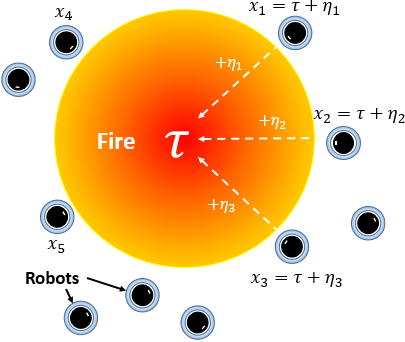
\includegraphics[width=\columnwidth]{../figures/globalgamesetup.png}
	\centering\caption{A multi-agent fire fighting scenario set up as a global game. Each player's imperfect estimate of the task is represented by $x_i$, a sum of the global magnitude parameter-$\tau$ and noisy sensor measurements-$\eta_i$.}\vspace{-10px}
\end{figure}

\newpage
\begin{figure}[!ht]
	\centering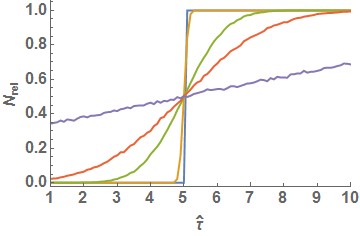
\includegraphics[width=\columnwidth]{../figures/thm2fig.png}
	\centering\caption{Visualization of Theorem~2 as $N_{rel}$ estimates $\Phi(\cdot)$. The plot was generated by running Eqn.~1 10,000 times for each point in $\hat{\tau} = 1$ to $10$ in increments of $0.1$. $n = 10$, $\td = 5$ and $x_i = \hat{\tau} + \eta_i$ ($\eta_i \sim\mathcal{N}(0, \sigma^2)$). Each curve in the plot is generated by sweeping $\sigma^2 = \{0, 0.1, 1, 2, 10\}$, with $\sigma^2 = 0$ being a step-function and $\sigma^2 = 10$ having the \emph{flattest} slope.}\label{fig:thm2fig}
\end{figure}
\end{document}